\section{How much is the given Autonomous Vehicle Parking scenario compliant to
GDPR?}

Privacy-enhancing technologies play an important role in preventing the
disclosure of private data as the information is transmitted and
processed~\cite[1-2]{10.1007/s10270-019-00718-z}.

We decided to limit the scope of our analysis to a subset of the provided flow.
More specifically, we omitted service registration and the parking itself, and
focused on the interaction with the parking service: from logging in to the
parking service to receiving a parking permit from the service. In effect, we
narrowed our scope to steps 5--17 of the full flow.

By analysing the provided flow (Figure~\ref{fig:initial-model}), we can
immediately identify some issues regarding GDPR compliance. For example, it is
unclear if the user is familiar with the privacy policy of the service, and how
data processing consent is given. Moreover, there seems to be no record of data
processing generated nor stored.

\begin{figure}[ht]
\begin{center}
  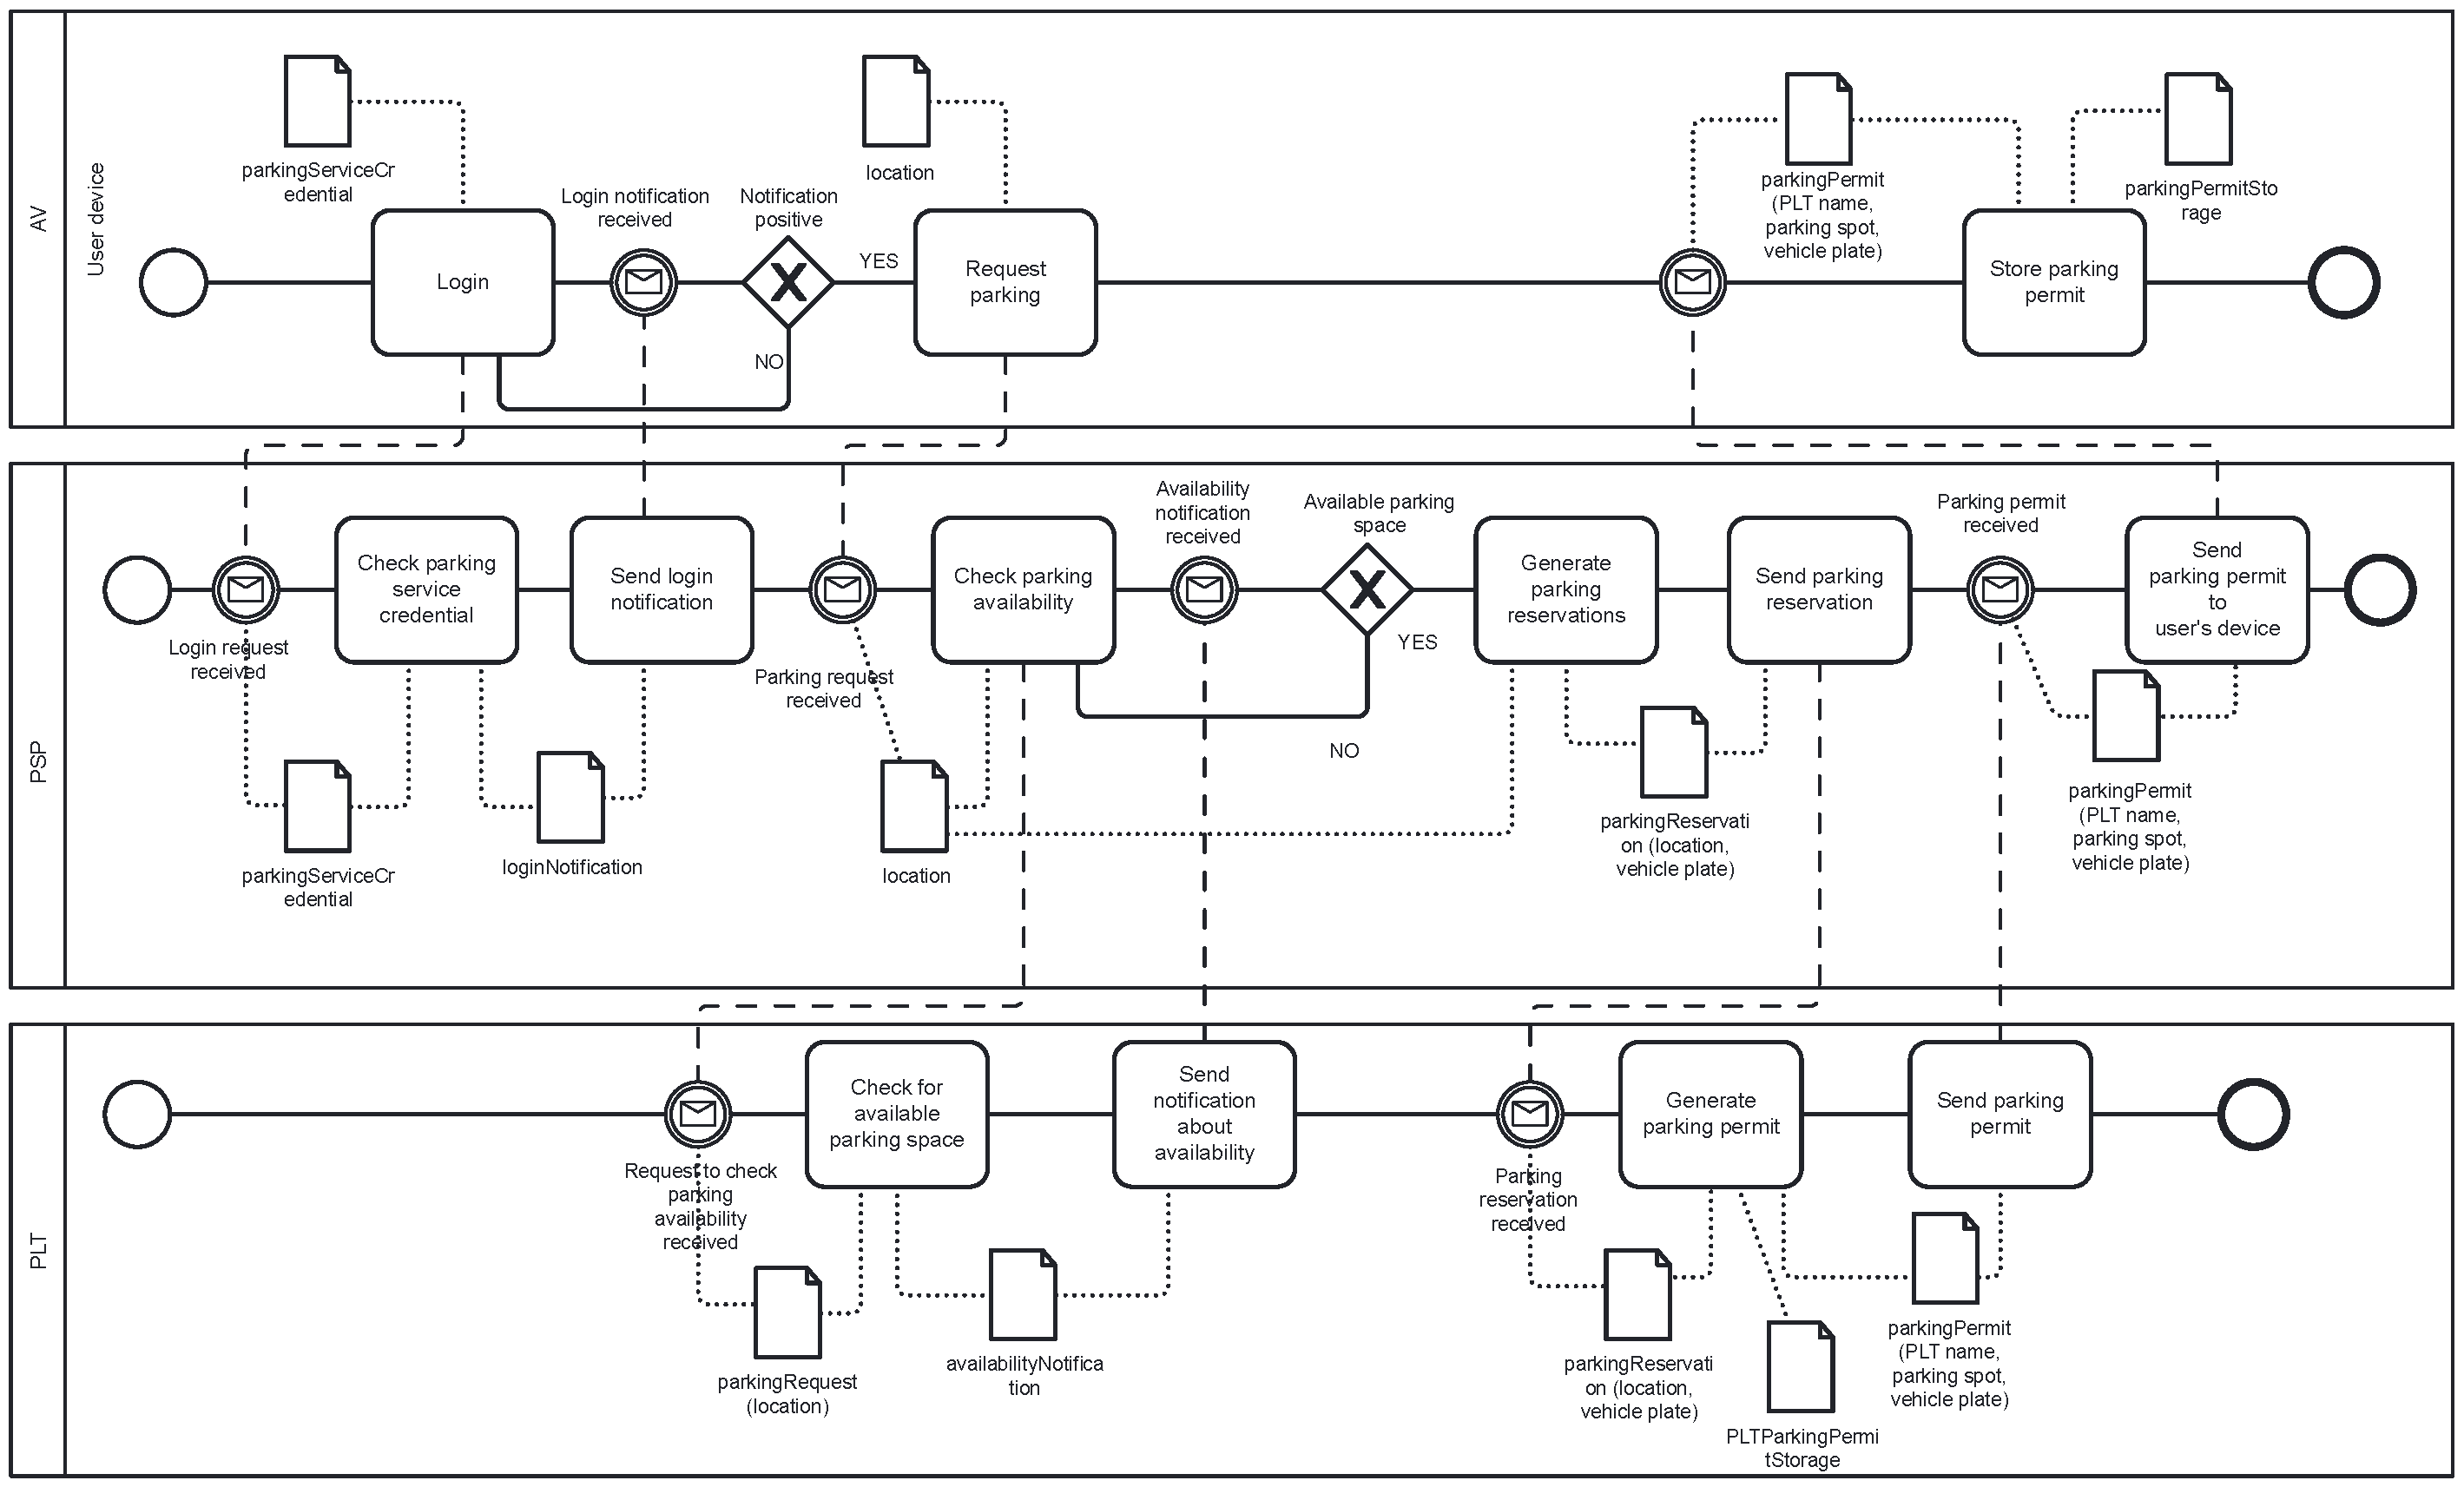
\includegraphics[width=\textwidth]{initial.pdf}
  \caption{Initial BPMN model (without GDPR annotations)}
  \label{fig:initial-model}
\end{center}
\end{figure}

The results of our analysis of the initial model with the DPO tool
(Figure~\ref{fig:initial-uml})~\cite{dpotool} revealed that several important
security measures are missing. These results align with our expectations because
of the aforementioned shortcomings, and the lack of GDPR annotations on the
model. Additionally, the analyses revealed the need for secure storage systems
to store the data and secure communication channels to transmit the data. All of
these measures are important to ensure compliance with privacy regulations and
to protect the privacy of personal data.


\begin{figure}[ht]
\begin{center}
  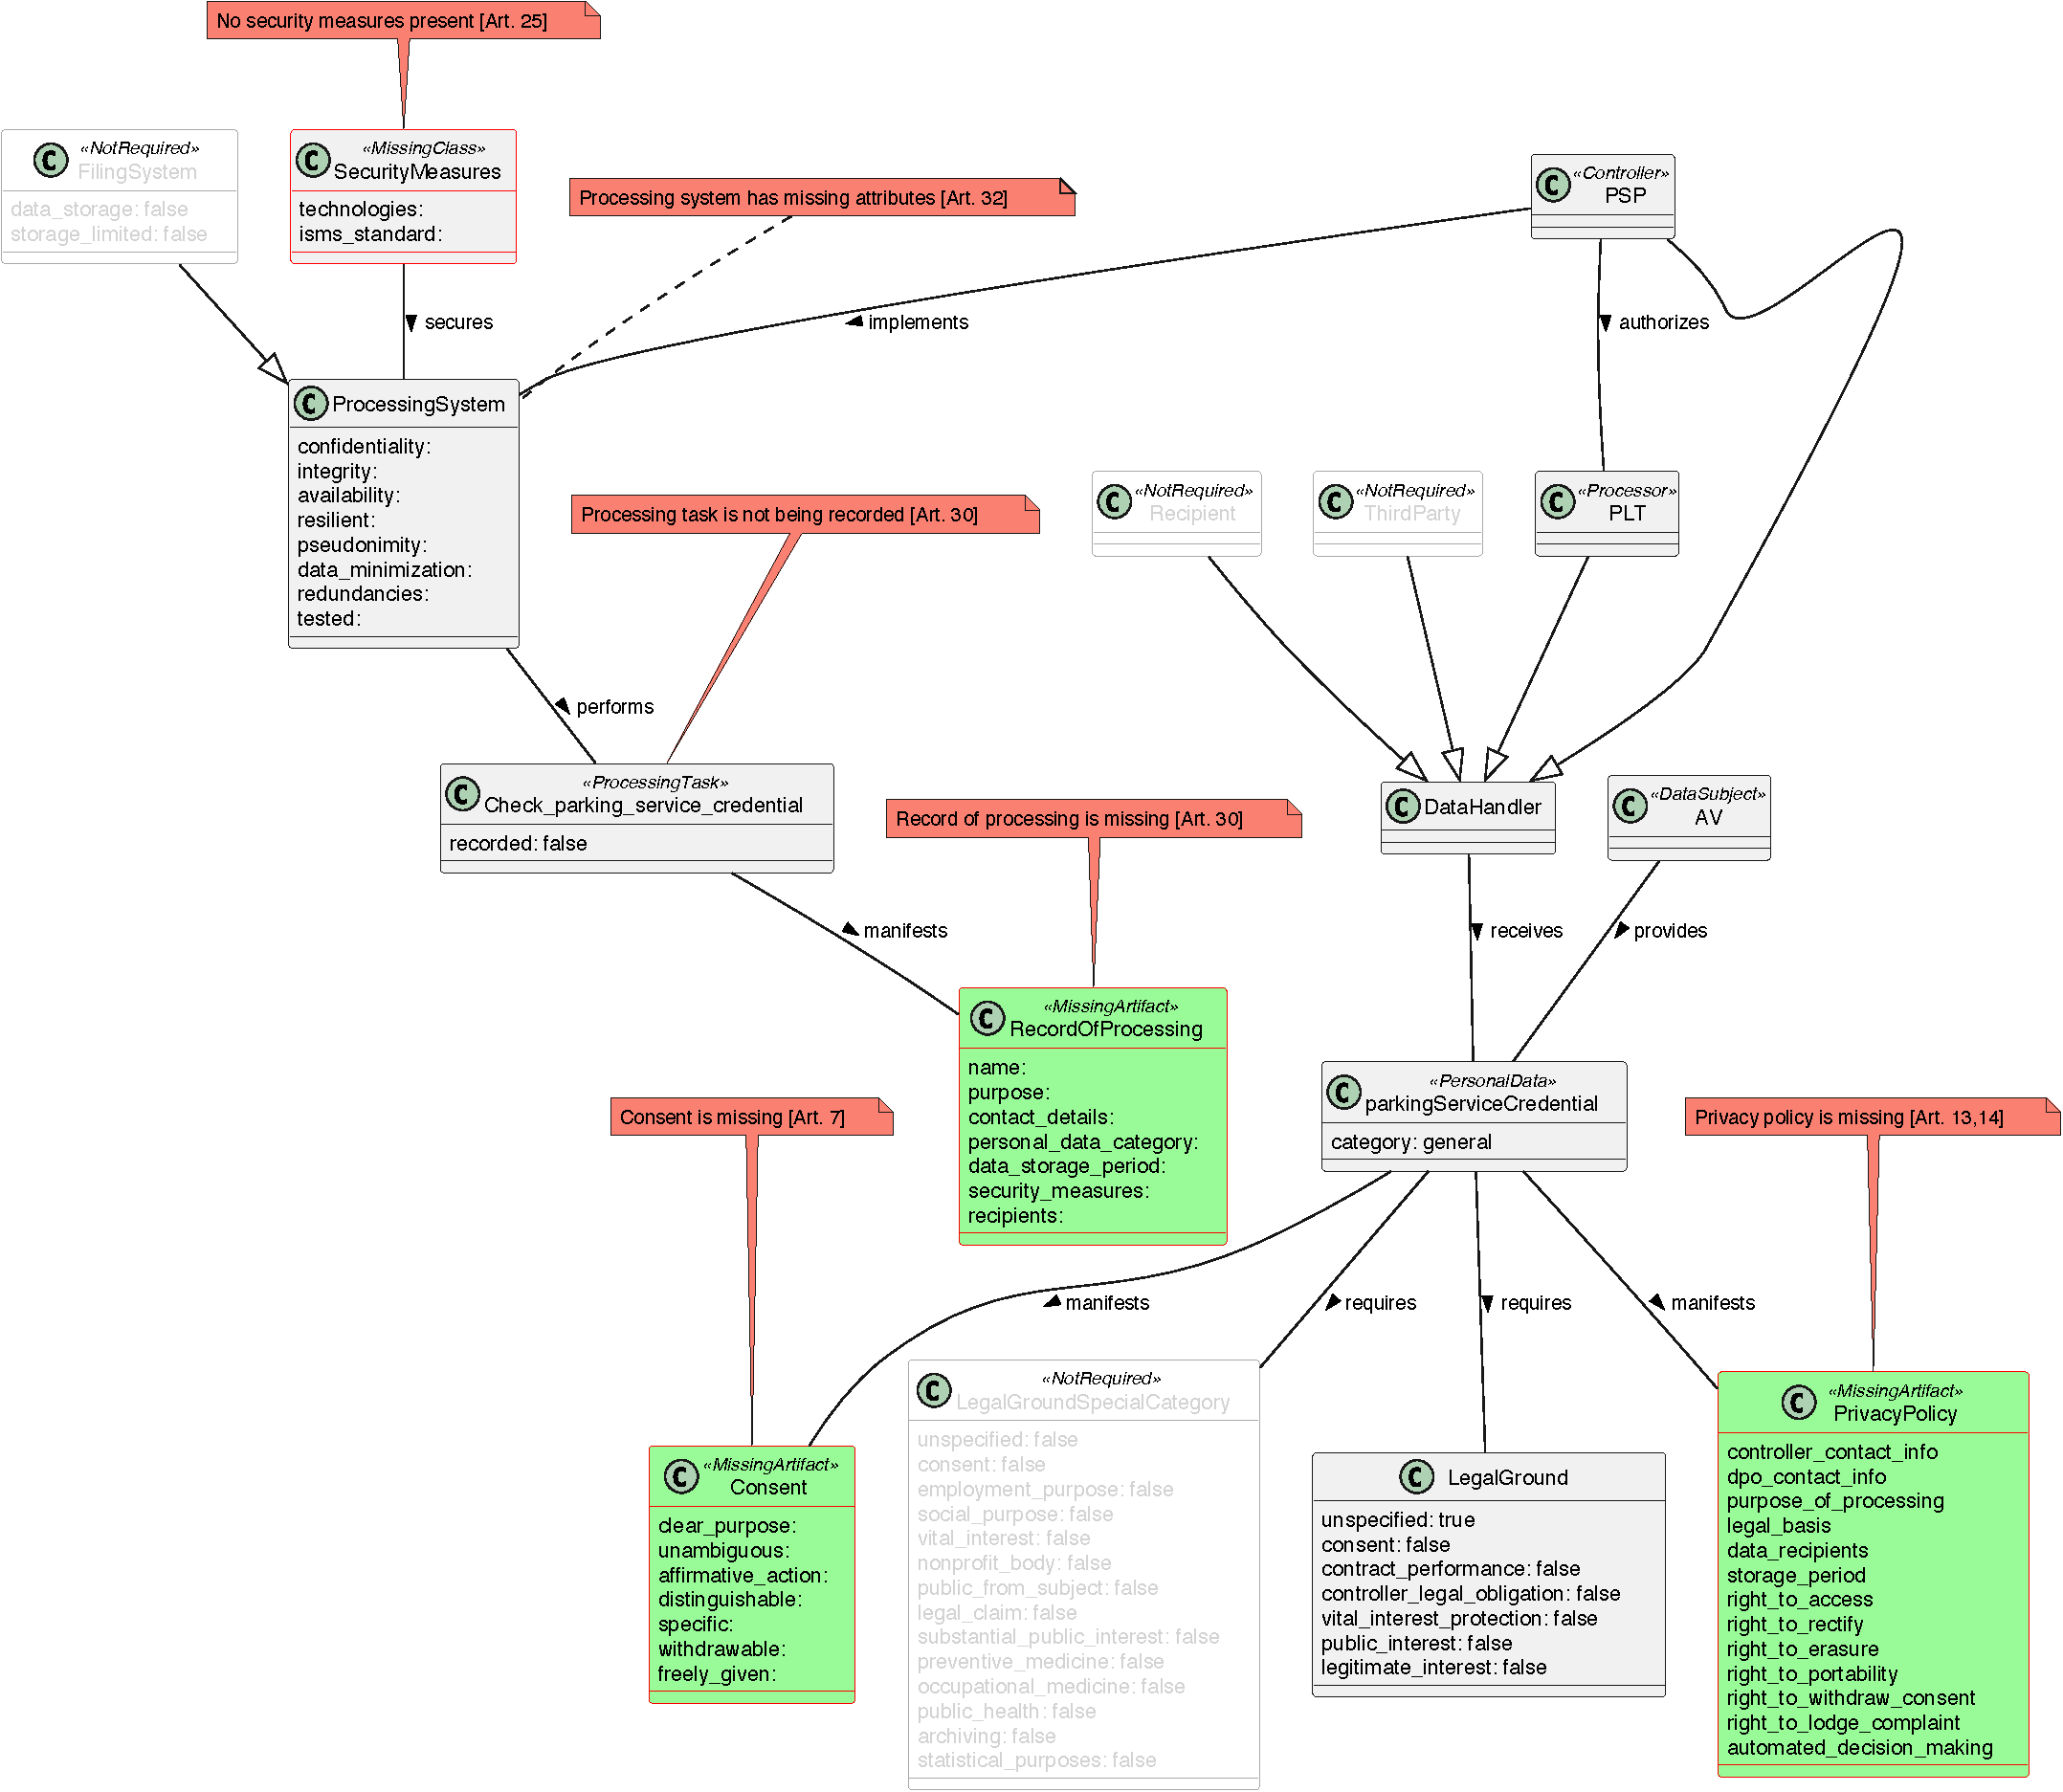
\includegraphics[width=\textwidth]{initial-uml.pdf}
  \caption{DPO tool analysis of the initial model}
  \label{fig:initial-uml}
\end{center}
\end{figure}

In summary, we identified the following aspects that are missing from the
scenario's model to make it GDPR compliant:
\begin{enumerate}
  \item no security measures present [Art. 25],
  \item the processing system has missing attributes [Art. 32],
  \item processing task is not being recorded [Art. 30],
  \item record of processing is missing [Art. 30],
  \item consent is missing [Art. 7],
  \item privacy policy is missing [Art. 13, 14].
\end{enumerate}
